\documentclass[12pt]{standalone}

%% for compilation with htlatex (to produce svg image),
%% uncomment the line below:
%\def\pgfsysdriver{pgfsys-tex4ht.def}

\usepackage{tikz}

\tikzstyle{tensor}=[rectangle,draw=blue!50,fill=blue!20,thick]
\tikzstyle{dots}=[thick]

\begin{document}

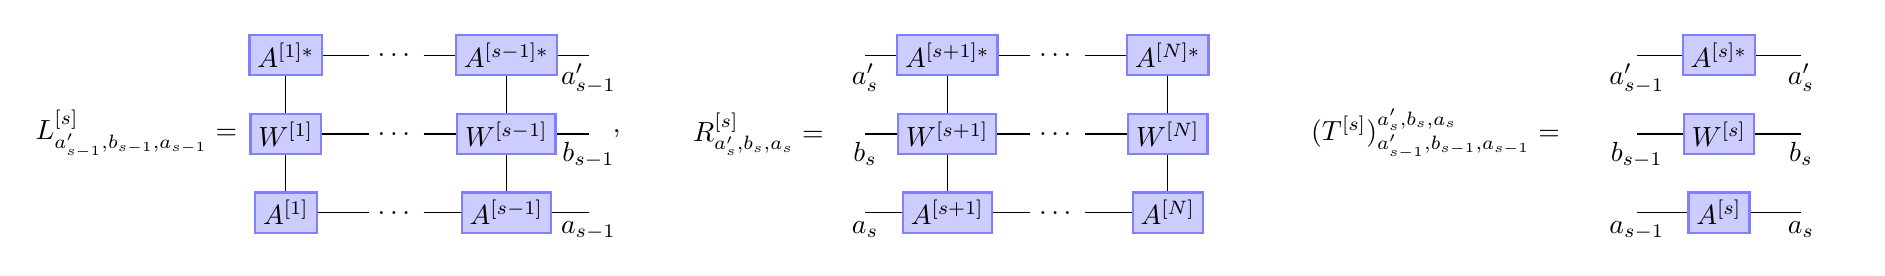
\begin{tikzpicture}[inner sep=1mm]
  \def\sep{1.4};
  %\def\x{1068}
  \node[tensor] (1 spin conjugate) at (\sep, 1.) {$A^{[1]*}$};
  \node[tensor] (1 spin) at (\sep, -1) {$A^{[1]}$};
  \node[tensor] (1) at (\sep, 0.) {$W^{[1]}$}; 

  \node[dots] (2 spin) at (2*\sep, -1) {\dots};
  \node[dots] (2 spin conjugate) at (2*\sep, 1) {\dots};
  \node[dots] (2) at (2*\sep, 0) {\dots};

  \node[tensor] (3 spin) at (3*\sep, -1) {$A^{[s-1]}$};
  \node[tensor] (3 spin conjugate) at (3*\sep, 1.) {$A^{[s-1]*}$};
  \node[tensor] (3) at (3*\sep, 0.) {$W^{[s-1]}$}; 

  \node[minimum width=0.7cm, minimum height=0.7cm] (4 spin) at (4*\sep,-1) {};
  \node[minimum width=0.7cm, minimum height=0.7cm] (4 spin conjugate) at
    (4*\sep,1.) {};
  \node[minimum width=0.7cm, minimum height=0.7cm] (4) at
    (4*\sep,0.) {,};




  \node[minimum width=0.7cm, minimum height=0.7cm] (5 spin) at (6*\sep, -1)
  {};
  \node[minimum width=0.7cm, minimum height=0.7cm] (5 spin conjugate) at
  (6*\sep, 1) {};
  \node[minimum width=0.7cm, minimum height=0.7cm] (5) at
  (6*\sep, 0) {};

  \node[tensor] (6 spin) at (7*\sep, -1) {$A^{[s+1]}$};
  \node[tensor] (6 spin conjugate) at (7*\sep, 1) {$A^{[s+1]*}$};
  \node[tensor] (6) at (7*\sep, 0.) {$W^{[s+1]}$};

  \node[dots] (7 spin) at (8*\sep, -1) {\dots};
  \node[dots] (7 spin conjugate) at (8*\sep, 1) {\dots};
  \node[dots] (7) at (8*\sep, 0.) {\dots};

  \node[tensor] (8 spin) at (9*\sep, -1) {$A^{[N]}$};
  \node[tensor] (8 spin conjugate) at (9*\sep, 1) {$A^{[N]*}$};
  \node[tensor] (8) at (9*\sep, 0.) {$W^{[N]}$};

  \foreach \x in {1,3, 6, 8} {
    \draw[-] (\x \space spin) -- (\x);
    \draw[-] (\x) -- (\x \space spin conjugate);
  }
  \foreach \x in {1, 6} {
    \pgfmathtruncatemacro{\xplusone}{\x + 1};
    \pgfmathtruncatemacro{\xplustwo}{\x + 2};
    \draw[-] (\x \space spin) -- ({\xplusone \space spin}.west);
    \draw[-] (\x \space spin conjugate) -- ({\xplusone \space spin conjugate}.west);
    \draw[-] ({\xplusone \space spin}.east) -- (\xplustwo \space spin);
    \draw[-] ({\xplusone \space spin conjugate}.east) 
      -- (\xplustwo \space spin conjugate);
    \draw[-] ({\xplusone}.east) -- (\xplustwo);
    \draw[-] ({\xplusone}.west) -- (\x);
  }

  %\draw (4 spin.north) node[right] {$\sigma_s$} -- (4 spin conjugate.south)
  %node[right] {$\sigma_s'$};
  
  \draw (3 spin) -- (4 spin.west) node[below] {$a_{s-1}$};
  \draw (3 spin conjugate) -- (4 spin conjugate.west) node[below] {$a_{s-1}'$};
  \draw (3) -- (4.west) node[below] {$b_{s-1}$};

  \draw (6 spin) -- (5 spin.east) node[below] {$a_{s}$};
  \draw (6 spin conjugate) -- (5 spin conjugate.east) node[below] {$a_{s}'$};
  \draw (6) -- (5.east) node[below] {$b_{s}$};
  %\draw (3 spin conjugate) -- (4 spin conjugate.west) node[above] {$a_{s-1}'$};
  %\draw (5 spin conjugate) -- (4 spin conjugate.east) node[above] {$a_{s}'$};

  \node at (-.5, 0.) {$L^{[s]}_{a_{s-1}', b_{s-1},a_{s-1}} = $};
  \node at (7.4, 0.) {$R^{[s]}_{a_{s}', b_{s},a_{s}} = $};


  \node[minimum width=0.7cm, minimum height=0.7cm] (T1 spin) at (13*\sep, -1) {};
  \node[minimum width=0.7cm, minimum height=0.7cm] (T1 spin conjugate) at (13*\sep, 1) {};
  \node[minimum width=0.7cm, minimum height=0.7cm] (T1) at (13*\sep, 0) {};

  \node[tensor] (T2 spin) at (14*\sep, -1) {$A^{[s]}$};
  \node[tensor] (T2 spin conjugate) at (14*\sep, 1.) {$A^{[s]*}$};
  \node[tensor] (T2) at (14*\sep, 0.) {$W^{[s]}$}; 

  \node[minimum width=0.7cm, minimum height=0.7cm] (T3 spin) at (15*\sep,-1) {};
  \node[minimum width=0.7cm, minimum height=0.7cm] (T3 spin conjugate) at
    (15*\sep,1.) {};
  \node[minimum width=0.7cm, minimum height=0.7cm] (T3) at
    (15*\sep,0.) {}; 

  \draw (T2 spin) -- (T1 spin.east) node[below] {$a_{s-1}$};
  \draw (T2 spin conjugate) -- (T1 spin conjugate.east) node[below] {$a_{s-1}'$};
  \draw (T2) -- (T1.east) node[below] {$b_{s-1}$};
  \draw (T2 spin) -- (T3 spin.west) node[below] {$a_{s}$};
  \draw (T2 spin conjugate) -- (T3 spin conjugate.west) node[below] {$a_{s}'$};
  \draw (T2) -- (T3.west) node[below] {$b_{s}$};
  \node at (16, 0.) {$(T^{[s]})_{a_{s-1}', b_{s-1},a_{s-1}}^{a_s',b_s,a_s} = $};
\end{tikzpicture}

\end{document}

